Here are some example where the distance is applied between the selected subset of articles and each year of the corpus:
\begin{figure}[H]
    \begin{minipage}[b]{0.3\linewidth}
        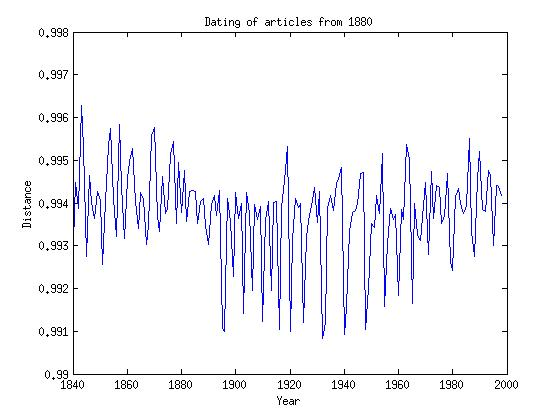
\includegraphics[scale=0.25]{Pictures/date_articles/distance1/dating1880.jpg}
        \caption{Dating articles from 1880 with the basic distance. Prediction is 1932.}
    \end{minipage}\hfill
    \begin{minipage}[b]{0.3\linewidth}
        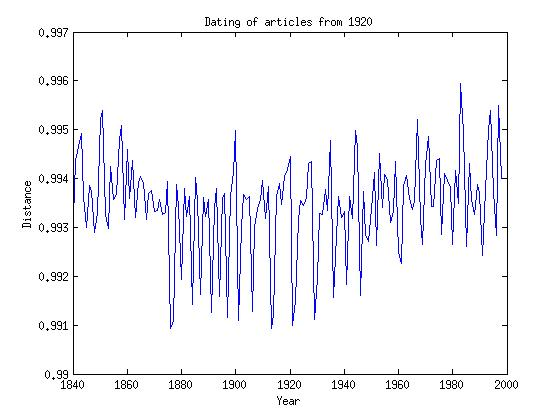
\includegraphics[scale=0.25]{Pictures/date_articles/distance1/dating1920.jpg}
        \caption{Dating articles from 1920 with the basic distance. Prediction is 1913.}
    \end{minipage}\hfill
    \begin{minipage}[b]{0.3\linewidth}
	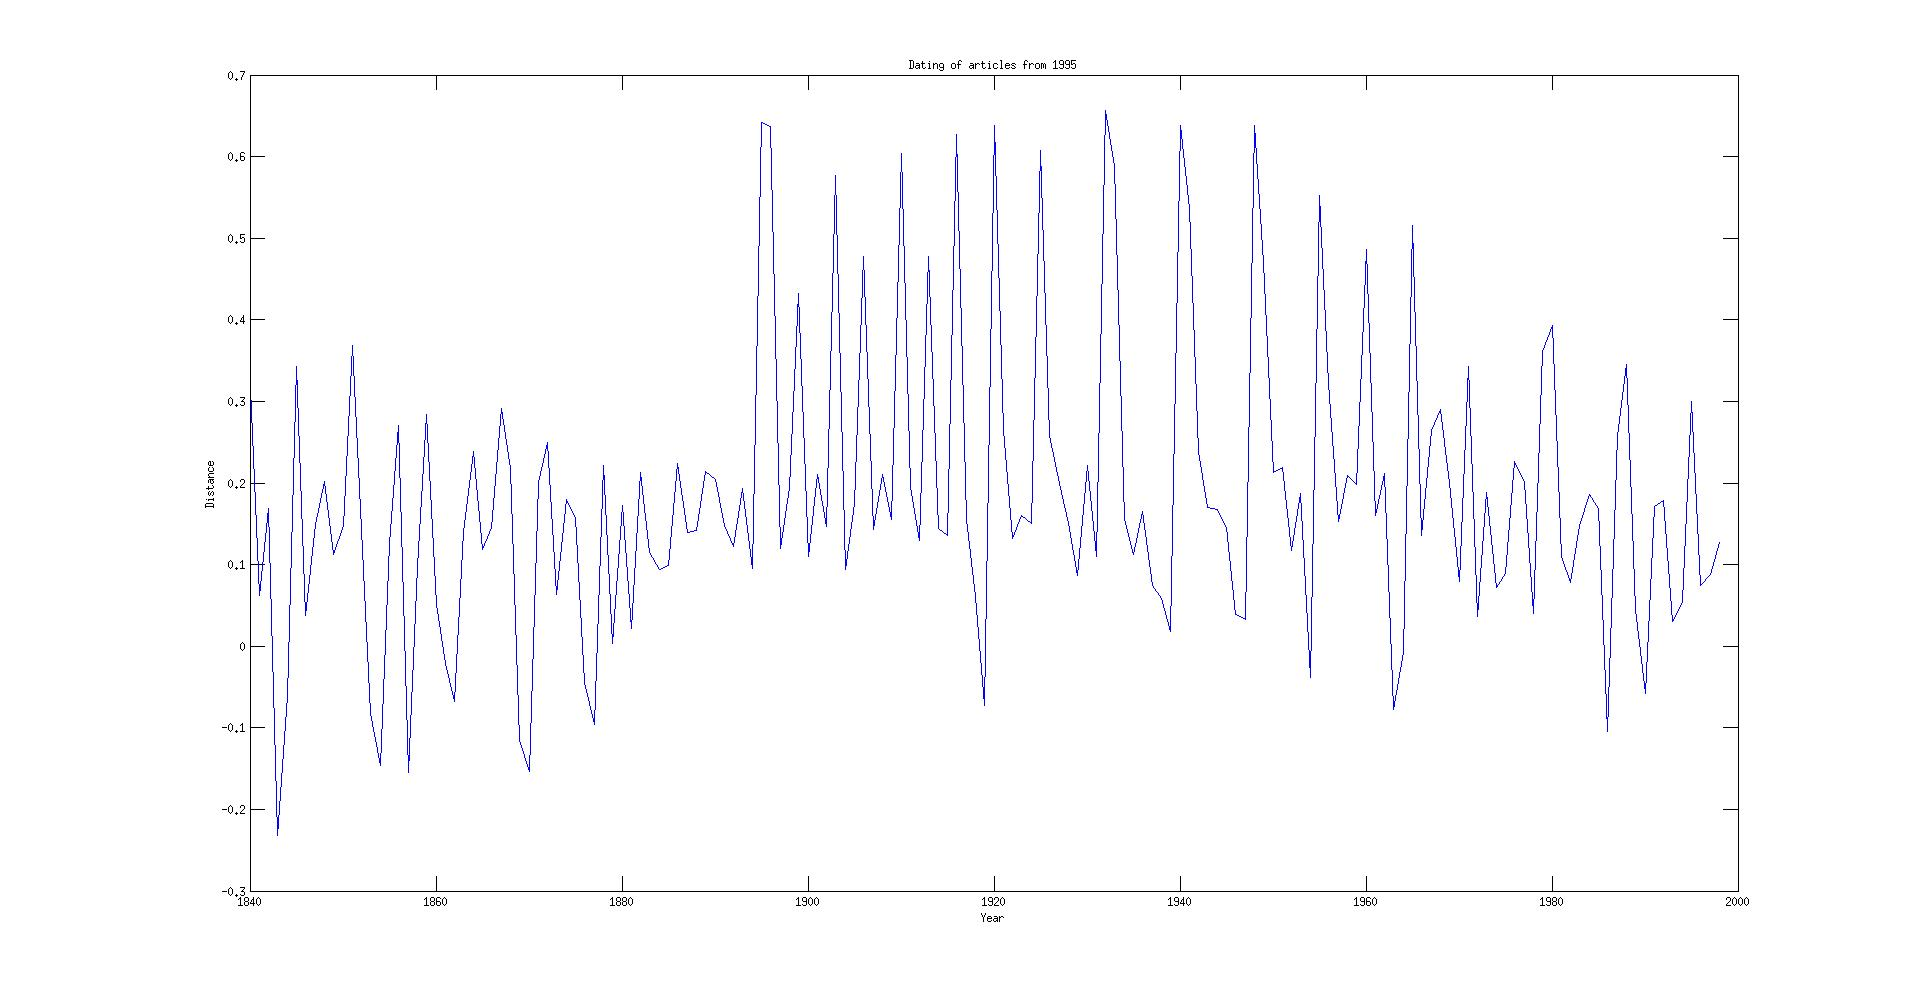
\includegraphics[scale=0.25]{Pictures/date_articles/distance1/dating1995_corrected.jpg}
        \caption{Dating articles from 1995 with the basic distance. Prediction is 1843.}
    \end{minipage}
\end{figure}
With the basic metric, the distances look very random, and the minimum doesn't give a good prediction. In our opinion, this "sawteeth" behavior can be explained because the amount of words suddenly drop in certain years. Indeed, the basic distance is subject to the number of words in each year and knowing that in 1840's years there are less words than in the others and that between 1917 and 1919 and in 1998 there are less articles too, the predicted year will almost always be one of the previous ones.
